\section{Analisi dei Carichi}\label{sec:loads}
 La trave in esame, che si trova al secondo impalcato (piano primo), è una trave perimetrale; le dimensioni della sezione, perciò, sono $30\times 50\,\si{cm}$ rispettivamente per la base e per l'altezza della trave.

\begin{figure}
 \centering
 \begin{tikzpicture}[scale=.7]
  \draw [thick, pattern=north east lines](-1.5, -2.5) rectangle (1.5, 2.5);
  \draw [|-|] (-1.5, -3.5) -- (1.5, -3.5) node at (0, -3.5) [anchor=south]{$30\,\si{cm}$} ;
  \draw [|-|] (-2, -2.5) -- (-2, 2.5) node at (-2, 0) [rotate=90, anchor=south]{$50\,\si{cm}$} ;
 \end{tikzpicture}
 \caption{Sezione della trave in cemento armato}
 \label{fig:beamSec}
\end{figure}

Come si può notare dalla figura~\ref{fig:pianoPrimo}, essendo la trave perimetrale, divide due ambienti: l'ambiente interno adibito ad uffici aperti al pubblico e il terrazzo esterno. Sarà, quindi,  necessario calcolare i carichi separatamente per la zona interna e per la zona esterna.

Nei seguenti paragrafi verranno elencati i carichi agenti sulla trave.

\subsection{Carichi permanenti strutturali}
Per quanto riguarda i carichi permanenti strutturali, questi si identificano nel \emph{peso proprio della trave} e nel \emph{peso proprio del solaio strutturale}; entrambi sono stati definiti nel capitolo~\ref{chap:intro}, rispettivamente pari a
\begin{equation*}
 G_{1k, t} = \gamma_{cls}\cdot B\cdot H = 25\,\dfrac{kN}{m^3} \cdot 0.30\,\si{m}\cdot 0.50\,\si{m} = 3.75\,\dfrac{kN}{m}
\end{equation*}
per la trave, dove $B$ è la base e $H$ è l'altezza della sezione. Mentre il peso del solaio strutturale è
\begin{equation*}
 g_{1k, solaio} = 3.20\,\dfrac{kN}{m^2}
\end{equation*}

\subsection{Carichi permanenti non strutturali}
Al contrario dei carichi strutturali, che in questo caso sono i medesimi e per il solaio interno e per il terrazzo, i carichi non strutturali si distinguono in funzione dell'ambiente.

\subsubsection*{Solaio interno}

\begin{align*}
 g_{2k, sottofondo} &= \gamma_{cls, all}\cdot s_{sottofondo} = 16\,\dfrac{kN}{m^3}\cdot 0.08\,\si{m} = 1.28\,\dfrac{kN}{m^2}\\
 g_{2k, massetto} &= \gamma_{massetto}\cdot
 s_{massetto} = 24\,\dfrac{kN}{m^3}\cdot 0.06\,\si{m} = 1.44\,\dfrac{kN}{m^2}\\
 g_{2k, pavimento} &= 0.50\,\dfrac{kN}{m^2}\\
 g_{2k, intonaco} &= \gamma_{intonaco}\cdot s_{intonaco} = 20\,\dfrac{kN}{m^3}\cdot 0.01\,\si{m} = 0.20\,\dfrac{kN}{m^2}
\end{align*}

Discorso diverso per quanto riguarda le divisorie interne. Il peso per unità di lunghezza della tramezza in laterizio è di 
\begin{align*}
 G_{2, div} &= \gamma_{div} \cdot s_{div} \cdot h_{div} + 2 \cdot \gamma_{intonaco} \cdot s_{intonaco} \cdot h_{div} =\\ &= 8.00\,\dfrac{kN}{m^3}\cdot 0.08\,\si{m} \cdot (3.10 - 0.25)\,\si{m} + 20\,\dfrac{kN}{m^3}\cdot 0.01\,\si{m} \cdot (3.10 - 0.25 - 0.01)\,\si{m}=\\ &= 2.96\,\dfrac{kN}{m}
 \end{align*}
 
 La normativa consente di convertire il carico per unità di lunghezza  delle divisorie in un carico uniformemente distribuito su un'area. Per elementi divisori con $2<G_2 \geq 3\,kN/_m$ si ha
 \[
  g_{2k, div} = 1.20\,\dfrac{kN}{m^2}
 \]
 
 In definitiva, per il solaio interno, i carichi permanenti non strutturali valgono
 \begin{align*}
	g_{2k, interno} &= g_{2k, sottofondo} + g_{2k, massetto} + g_{2k, pavimento} + g_{2k, intonaco} + g_{2k, div}=\\ &= (1.28 + 1.44 + 0.50 + 0.20 + 1.20)\,\dfrac{kN}{m^2} =\\&=
	4.62\,\dfrac{kN}{m^2}
 \end{align*}
 
 \subsubsection*{Solaio terrazza}
 Il solaio della terrazza si distingue da quello interno principalmente per la pavimentazione e per la presenza dell'solante termico.

\begin{align*}
 g_{2k, isolante} &= \gamma_{isolante}\cdot s_{isolante} = 0.50\,\dfrac{kN}{m^3}\cdot 0.15\,\si{m} = 0.075\,\dfrac{kN}{m^2}\\
 g_{2k, massetto} &= \gamma_{massetto}\cdot s_{massetto} = 24\,\dfrac{kN}{m^3}\cdot 0.06\,\si{m} = 1.44\,\dfrac{kN}{m^2}\\
 g_{2k, pavimento} &= 0.50\,\dfrac{kN}{m^2}\\
 g_{2k, intonaco} &= \gamma_{intonaco}\cdot s_{intonaco} = 20\,\dfrac{kN}{m^3}\cdot 0.01\,\si{m} = 0.20\,\dfrac{kN}{m^2}
\end{align*}

Sommando i contributi dei singoli carichi distribuiti si ottiene il valore finale per la terrazza
 \begin{align*}
	g_{2k, terrazza} &= g_{2k, isolante} + g_{2k, massetto} + g_{2k, pavimento} + g_{2k, intonaco} =\\ &= (0.075 + 1.44 + 0.50 + 0.20)\,\dfrac{kN}{m^2} =\\&=
	2.215\,\dfrac{kN}{m^2}
 \end{align*}

\subsubsection*{Tamponamenti perimetrali}
Il peso della muratura perimetrale ricade nei carichi permanenti non strutturali. Secondo quanto descritto nel capitolo~\ref{chap:intro}, la stratigrafia della parete è quella rappresentata in figura~\ref{fig:stratigrafiaTamponamento}

\begin{figure}
 \centering
 \begin{tikzpicture}[scale=.5]
  \draw (0,0) rectangle (3, 10);
    \foreach \y in {0, .4, ..., 10}
	\draw (0, \y) -- (3, \y);
	
	\foreach \x in {0, .4, ..., 3}
		\draw (\x, 0) -- (\x, 10);

\node at (1.5, 5) [fill=white, rotate=90] {$laterizio$};

 \draw [fill=black] (3,0) rectangle (3.1, 10);
 \draw [->, thin] (3.05, 5) -- +(1, 0) node [anchor = west] {$intonaco$};
 
 \draw[pattern=north east lines] (0,0) rectangle (-1.2, 10);
 \node at (-.6, 5) [fill=white, rotate=90] {$cappotto$};
 
 \draw[|-|, thin] (-1.2, -2) -- (0, -2);\draw[-|, thin] (0, -2) -- (3, -2); \draw[-|, thin](3, -2) -- (3.1, -2);
 \node at (-.6, -1.8) [anchor=south] {$12\si{cm}$};
  \node at (1.5, -1.8) [anchor=south] {$30\si{cm}$};
   \node at (3.2, -1.8) [anchor=south] {$1\si{cm}$};
 \end{tikzpicture}
 \caption{Stratigrafia tamponamento perimetrale}
 \label{fig:stratigrafiaTamponamento}
\end{figure}

Il carico, che risulterà essere distribuito lungo una linea e gravante direttamente sulla trave, ha valore
\begin{align*}
 G_{2k, tamp} &= \gamma_{tamp} \cdot s_{tamp} \cdot h_{piano} + \gamma_{cappotto} \cdot s_{cappotto} \cdot h_{piano} + \gamma_{intonaco} \cdot s_{intonaco} \cdot h_{piano} =\\
 &= \left(10\,\dfrac{kN}{m^3}\cdot 0.30\,\si{m} + 0.20\,\dfrac{kN}{m^3}\cdot 0.12\,\si{m} + 20\,\dfrac{kN}{m^3}\cdot 0.01\,\si{m}\right)\cdot 2.85\,\si{m} = 9.20\,\dfrac{kN}{m}
\end{align*}


\subsection{Carichi variabili}
Come già detto in precedenza, la trave è una trave perimetrale che divide due ambienti: un ambiente interno adibito a uffici aperti al pubblico e una terrazza esterna soggetta alle azioni meteorologiche. Si ha la necessità, anche in questo caso, di suddividere i carichi variabili dei due differenti ambienti.

\subsubsection*{Solaio interno}
Il solaio interno deve essere progettato per sostenere degli uffici aperti al pubblico. Seguendo quanto descritto nelle \emph{NTC 2018}, in particolare nella \textbf{Tab. 3.1.II}, la categoria in cui si ricade è la \emph{B2}. 

Si deduce che il valore del sovraccarico è di 
\[
 q_{k, CAT.\,B2} = 3\,\dfrac{kN}{m^2}
\]

\subsubsection*{Terrazza}
Sul solaio della terrazza si deve tener conto e del carico variabile della categoria definita sopra (con riferimento al valore per \emph{balconi} e \emph{ballatoi}) e delle azioni dei fenomeni meteorologici quali neve e vento. In ordine si trova
\[
 q_{k, CAT.B}^{balconi} = 4\,\dfrac{kN}{m^2}
\]

\paragraph{Carico neve}

Il carico dovuto alla neve è calcolato seguendo quanto scritto nel \textbf{capitolo 3.4} delle \emph{NTC 2018}. In particolare, la \emph{[3.4.1]} definisce il carico provocato dalla neve sulla copertura
\[
 q_s = q_{sk}\cdot \mu_i \cdot C_E \cdot C_t
\]

L'edificio si trova in \emph{Provincia di Trento}, il che ricade nella zona di carico neve \textbf{'I - Alpina'} che gli conferisce un carico di neve al suolo pari a
\begin{align*}
 q_{sk} = 
 \begin{cases}
    1.50\,\dfrac{kN}{m^2}\quad &\text{se } a_s < 200\,\si{m}\\\\
    1.39\,\left[ 1 + \left(\dfrac{a_s}{728}\right)^2\right]\,\left[\dfrac{kN}{m^2}\right]\quad &\text{se } a_s > 200\,\si{m}
 \end{cases}
\end{align*}

L'altitutide è $788\,\si{m} > 200\,\si{m}$ per cui

\[
 q_{sk} = 1.39\,\left[ 1 + \left(\dfrac{788}{728}\right)^2\right] = 3.02\,\dfrac{kN}{m^2}
\]

Poiché non sono presenti informazioni riguardo la localizzazione e quindi l'esposizione dell'edificio al vento che produrrebbe una rimozione della neve sulla copertura, si considera la topografia dell'area \emph{normale}, cioè si assume
\[
 C_E = 1
\]

Inoltre, non avendo documenti che descrivono il fenomeno di scioglimento della neve causato dal riscaldamento prodotto all'interno dell'edifico, si assume cautelativamente il coefficiente termico unitario
\[C_t = 1\]

Come riportato nella \emph{circolare n. 7 del 2019} al \textbf{capitolo C3.4.3}, nel caso in esame si devono considerare due diversi coefficienti di forma per la copertura:
\begin{itemize}
	\item coefficiente di forma per copertura piana
	\[
		\mu_1 = 0.8
	\]
	\item coefficiente di forma per copertura adiacente o vicina a costruzioni più alte (\textbf{capitolo C3.4.3.3.2}).
\end{itemize}

Nel secondo caso, la circolare considera un effetto dovuto allo scivolamento della neve dalla copertura (inclinata) posta a quota superiore ($\mu_s$) e un effetto di deposito, dovuto al vento, in corrispondenza della parete verticale che delimita le due coperture ($\mu_w$) come si può vedere in figura~\ref{fig:muCircolare}.

\begin{figure}
 \centering
 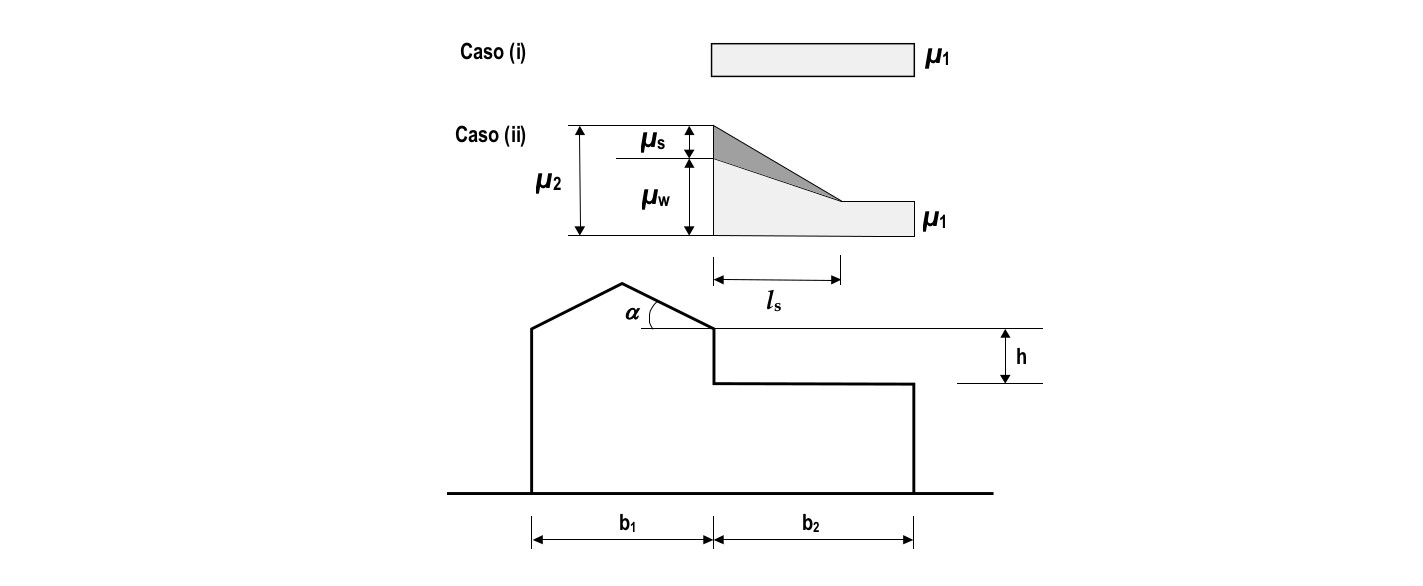
\includegraphics[width=\textwidth]{muCircolare}
  \caption{Coefficienti di forma per il carico neve per coperture adiacenti a costruzioni più alte (\emph{circolare n. 7 - 2019})}
  \label{fig:muCircolare}
\end{figure}


Poiché la copertura superiore è piana, la quota parte dello scivolamento risulta non esserci; di conseguenza si assume
\[
	\mu_s = 0
\]

Al contrario è presente il contributo dovuto all'accumulo che è calcolato come segue
\begin{align*}
 \mu_2 &= \mu_s + \mu_w = \mu_w\\
 \mu_w &=  \dfrac{b_1 + b_2}{2 h}\leq \gamma_{snow}\,\dfrac{h}{q_{sk}}
\end{align*}
dove $\gamma_{snow} = 2\,kN/_{m^3}$ è il peso per unità di volume della neve. Inoltre la normativa impone che 
\[
 0.8 \leq \mu_w \leq 4.0
\]

Nel caso in esame il coefficiente vale
\[
 \mu_w =  \dfrac{b_1 + b_2}{2 h} = \dfrac{18+6}{2\cdot 2} = 1.94 < \dfrac{2\cdot 6.2}{3.02} = 4.11
\]
e inoltre $\mu_w \in [0.8, 4.0]$.


Come rappresentato in figura~\ref{fig:muCircolare}, la lunghezza in cui si forma l'accumulo è
\[
 l_s = 2 h, \quad 5\,m\leq l_s \leq 15\,m
\]

Cioè

\begin{align*}
  &l_s = 2 h = 2\cdot 6.2\,m = 12.4\,m > b_2 = 6\,m\\
  &l_s \in [5, 15]\,m
\end{align*}

Il coefficiente di accumulo sul bordo del terrazzo va calcolato interpolando linearmente; la generica interpolazione è
\[
 \dfrac{x-x_0}{x_1-x_0} = \dfrac{y-y_0}{y_1-y_0}
\]

Sostituendo $(x_0, y_0) = (0, 1.94)$ e $(x_1, y_1) = (12.4, 0.8)$, nonché $x = 6$, si ottiene che
\[ 
 y = \dfrac{6}{12.4}\,(0.8-1.94) + 1.94 = 1.38
\]
nella zona dove la terrazza ha larghezza $6\,m$, come rappresentato in figura; mentre
\[
 y = \dfrac{3.5}{12.4}\,(0.8-1.94) + 1.94 = 1.62
\]
dove la terrazza ha larghezza pari a $3.50\,m$.







\begin{figure}
	\centering
	\subfloat[\emph{Coefficienti di forma per il tratto di terrazza di larghezza $6\,m$}]{
	\begin{tikzpicture}[scale=.8]
		\draw (0,0) -- (0,2) -- (10,2) -- (10, 6) -- (12, 6);
		\draw [thick, pattern=north east lines] (0,2.5) --  (9.5, 2.5) -- ++(0, 2.4) -- (0,3.3) --cycle; 
		\node at (0,3.3) [anchor = north east] {$\mu_1 = 1.38$};
		\node at (9.5, 4.9) [anchor = south east] {$\mu_w = 1.94$};
		
		\draw [<->] (11, 2) -- (11, 6) node at (11, 4) [anchor =south, rotate = 90] {$h$};
		\draw [<->] (0,1) -- (10,1) node at (5,1) [anchor = south] {$b_2 = 6.0\,m$};
		\draw [<-] (10,1) -- (11,1);
		\draw [-, dashed] (11,1) -- (12,1);
		\node at (11, 1) [anchor = south] {$b_1 = 6.2\,m$};
	\end{tikzpicture}}\\
	\subfloat[Coefficienti di forma per il tratto di terrazza di larghezza $3.5\,m$]{\begin{tikzpicture}[xscale=.4, yscale=.8]
		\draw (0,0) -- (0,2) -- (10,2) -- (10, 6) -- (14, 6);
		\draw [thick, pattern=north east lines] (0,2.5) --  (9.5, 2.5) -- ++(0, 2.4) -- (0,3.3) --cycle; 
		\node at (0,3.3) [anchor = north east] {$\mu_1 = 1.62$};
		\node at (9.5, 4.9) [anchor = south east] {$\mu_w = 1.94$};
		
		\draw [<->] (12, 2) -- (12, 6) node at (12, 4) [anchor =south, rotate = 90] {$h$};
		\draw [<->] (0,1) -- (10,1) node at (5,1) [anchor = south] {$b_2 = 3.5\,m$};
		\draw [<-] (10,1) -- (12,1);
		\draw [-, dashed] (12,1) -- (14,1);
		\node at (12, 1) [anchor = south] {$b_1 = 6.2\,m$};
	\end{tikzpicture}}
    \caption{Descrizione grafica dell'andamento lineare dei coefficienti di forma}
    \label{fig:muTerrazza_6m}
\end{figure}

Il coefficiente $\mu_2$ è calcolato come la media tra i due coefficienti $\mu_1$ e $\mu_w$
\begin{equation*}
 \begin{cases}
  \mu_{2,1} = \dfrac{1.94 + 1.38}{2} = 1.66\\\\
  \mu_{2,2} = \dfrac{1.94+1.62}{2} = 1.78
 \end{cases}
\end{equation*}

Il carico da neve sul tratto di larghezza $6\,m$ è 
\begin{equation}
\label{eq:neve_1}
 \begin{cases}
  q_{s,1}^{(1)} = q_{sk}\cdot \mu_1 \cdot C_E\cdot C_t = 3.02\,\dfrac{kN}{m^2}\cdot 0.8\cdot 1\cdot 1 = 2.41\,\dfrac{kN}{m^2}\\\\
  q_{s,1}^{(2)} = q_{sk}\cdot \mu_{2,1} \cdot C_E\cdot C_t = 3.02\,\dfrac{kN}{m^2}\cdot 1.38\cdot 1\cdot 1 = 4.17\,\dfrac{kN}{m^2}
 \end{cases}
\end{equation}
mentre per il tratto di $3.5\,m$
\begin{equation}
 \label{eq:neve_2}
 \begin{cases}
  q_{s,2}^{(1)} = q_{sk}\cdot \mu_1 \cdot C_E\cdot C_t = 3.02\,\dfrac{kN}{m^2}\cdot 0.8\cdot 1\cdot 1 = 2.41\,\dfrac{kN}{m^2}\\\\
  q_{s,2}^{(2)} = q_{sk}\cdot \mu_{2,2}\cdot C_E\cdot C_t = 3.02\,\dfrac{kN}{m^2}\cdot 1.62\cdot 1\cdot 1 = 4.90\,\dfrac{kN}{m^2}
 \end{cases}
\end{equation}


\paragraph{Carico vento}

Il carico derivante dal vento è normato nel \textbf{capitolo 3.3} delle \emph{NTC 2018} dove si ha una suddivisione del territorio nazionale in zone. La Provincia di Trento ricade in \textbf{zona 1} in cui i valori dei parametri da utilizzare nel calcolo derivano dall \textbf{Tab. 3.3.I} e sono
\begin{equation*}
 \begin{cases}
    v_{b,0} = 25\,\dfrac{m}{s}\\
    a_0 = 1000\,m\\
    k_s = 0.40
 \end{cases}
\end{equation*}
dove $v_{b,0}$ è la velocità base di riferimento al livello del mare. Si ricava la velocità di riferimento (valore medio su $10$ minuti ad un'altezza di $10\,m$ dal suolo) come
\[
 v_b = v_{b,0}\cdot c_a
\]
dove $c_a$ è il coefficiente di altitutide che, nell'oggetto in studio vale
\[
 c_a = 1, \quad \text{per } a_s = 788\,m < a_0 = 1000\,m
\]

Allora
\[
 v_b = v_{b,0} = 25\,\dfrac{m}{s}
\]

Con riferimento ad un tempo di ritorno pari a $50\,anni$ ($c_r(T_r=50\,anni) = 1$), la velocità di riferimento è
\[
 v_r = v_b\cdot c_r = 25\,\dfrac{m}{s}
\]

Con i dati finora calcolati è possibile valutare la pressione del vento, assumendo la densità dell'aria di $1.25\,kg/_{m^3}$
\[
 q_{cin} = \dfrac{1}{2}\cdot\rho\, v_r^2 = \dfrac{1}{2}\,1.25\,\dfrac{kg}{m^3}\cdot\left(25\,\dfrac{m}{s}\right)^2 = 390.625\,Pa
\]

La pressione del vento è quindi data dalla seguente formula (\emph{[3.3.4]})
\[
 p = q_{cin}\cdot c_e\cdot c_p\cdot c_d
\]

Il coefficiente di esposizione $c_e$ dipende da vari parametri come l'altezza dal suolo, la topografia dell'area e dalla categoria di esposizione. Quest'ultima in particolare è assegnata dalla \textbf{Tab. 3.3.III}. Ipotizzando che l'edificio si trovi in area industriale suburbana, la classe di rugosità del terreno risulta essere la \textbf{B}; inoltre, ci si trova ad una distanza dal mare superiore a $30\,km$ e ad un'altitudine di $788\,m > 750\,m$, perciò, dalla \textbf{Fig. 3.3.2} si deduce che la categoria di esposizione è la \textbf{IV} che fornisce i seguenti parametri per il calcolo del coefficiente di esposizione
\begin{equation*}
 \begin{cases}
    k_r = 0.22\\
    z_0 = 0.30\,m\\
    z_{min} = 8\,m
 \end{cases}
\end{equation*}

L'altezza totale dell'edificio è di $9.7\,m$ che risulta essere superiore alla $z_{min} = 8\,m$. Come specificato nella \emph{[3.3.7]} il coefficiente di esposizione va calcolato come
\begin{align*}
 c_e(z) &= k_r^2 \, c_t\,\ln\left(\dfrac{z}{z_0}\right)\,\left[ 7 + c_t\,\ln\left(\dfrac{z}{z_0}\right)\right] = \\
 &= 0.22^2 \cdot 1\cdot \ln\left(\dfrac{9.70}{0.30}\right)\,\left[ 7 + 1\cdot\ln\left(\dfrac{9.70}{0.30}\right)\right] = 1.76
\end{align*}
in cui si è assunto il coefficiente di topografia $c_t = 1$, come consigliato nella normativa.

Cautelativamente si assume anche il coefficiente dinamico unitario $c_d = 1$.

Per quanto riguarda il calcolo del coefficiente di pressione $c_p$ si fa riferimento alla \emph{circolare n.7 2019}, in particolare al \textbf{capitolo C3.3.8.1.2} in cui vengono trattate le coperture piane.

\begin{figure}
 \centering
 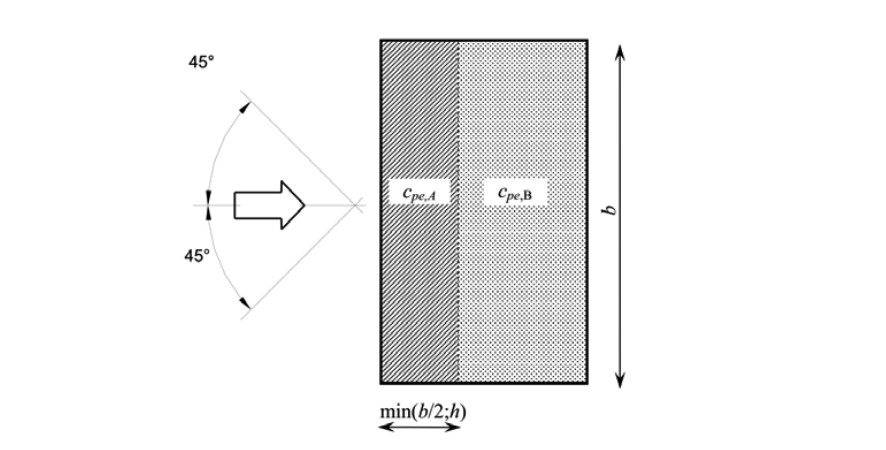
\includegraphics[width=\textwidth]{pressureCoeff}
 \caption{Schema di riferimento per il calcolo del coefficiente di pressione su coperture piane (\emph{Fig. C3.3.5})}
 \label{fig:pressureCoeff_circolare}
\end{figure}

Come si può notare in figura~\ref{fig:pressureCoeff_circolare}, l'effetto generato dal vento cambia in funzione che questo arrivi da destra o da sinistra. In particolare, se il vento spira da sinistra verso destra si ha un effetto di depressione, favorevole alla sicurezza, 'alleggerendo' la struttura; se invece spira in direzione opposta può avere sia un effetto di pressione che di depressione (zona B della figura). Il coefficiente di pressione in quest'ultimo caso è
\[
 c_{pe,B} = \pm 0.20
\]
essendo la terrazza in esame in zona B, poiché
\[ 
 min \left\{\dfrac{b}{2}; h\right\} = min \left\{\dfrac{28}{2}; 9.7\right\} = 9.7\,m
\]

L'effetto ricercato per le massime sollecitazioni agenti è quello di pressione (segno positivo), mentre per valutare il minimo verrà utilizzato quello con segno negativo. 
La pressione, perciò, vale
\begin{equation}
\label{eq:windPressure}
 p = q_{cin}\cdot c_e\cdot c_p\cdot c_d = 390.625\,Pa \cdot 1.76\cdot (\pm 0.20) \cdot 1 = \pm 0.138\,\dfrac{kN}{m^2}
\end{equation}

\begin{table}
\caption{Riepilogo dei carichi agenti}  
\label{tab:azioni_trave}
 \begin{tabular}{lccccccr}
 \toprule
   &$g_{1k}\,[kN/_{m^2}]$ &$g_{2k}\,[kN/_{m^2}]$ & $q_{CAT. B2}\,[kN/_{m^2}]$&$q_{s}\,[kN/_{m^2}]$&$q_{w}\,[kN/_{m^2}]$\\
   \midrule
   Interno &$3.2$&$4.62$&$3.00$& &&&\\
   Terrazza &$3.2$&$2.215$&$4.00$&
   \begin{tabular}{c}
    $2.41$\\$4.17$\\$4.90$
   \end{tabular}
&$\pm 0.138$&&\\  
\midrule
&$G_{1k}\,[kN/_{m}]$&$G_{2k}\,[kN/_{m}]$\\
\midrule
    Trave&$3.75$&$9.20$&&&&&\\
  \bottomrule
 \end{tabular}
\end{table}

